\section{Theorie}
\label{sec:Theorie}

Eine Spannungsquelle kann eine konstante Leistung über einen endlichen Zeitraum
 hinweg erzeugen. Es wird von einer Leerlaufspannung $ U_0 $
an den Ausgangsklemmen gesprochen, falls der Spannungsquelle kein Strom entnommen wird.
Sobald es zu einer Leistungsabnahme durch einen äußeren Widerstand $ R_a $ kommt,
sinkt die an den Klemmen gemessene Spannung, die "Klemmenspannung", unter den Wert von $ U_0 $. Erklärt wird
dies durch einen Eigenwiderstand der Spannungsquelle. In der Theorie wird die reale
Spannungsquelle durch eine ideale Spannungsquelle in Reihe mit einem Widerstand $ R_i$
ersetzt.
\begin{figure}[H]
  \centering

  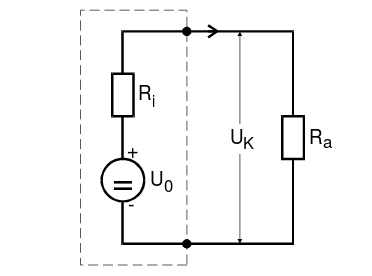
\includegraphics[width=\linewidth-200pt,height=\textheight-200pt,keepaspectratio]{content/Spannungsquelle1.png}
  \caption{Reale Spannungsquelle [1]}
  \label{fig:Spannung1}
\end{figure}

Aus dem zweiten kirchhoffschen Gesetz folgt dann gemäß Abb. 1
\begin{equation}
	 U_0 = I R_i + I R_a  \text{ bzw. } U_k = I R_a = U_0-IR_i
\end{equation}
Zur Messung der Leerlaufspannung wird deshalb ein hochohmiges Voltmeter verwendet,
sodass der Strom $I$ gegen $0$ läuft und somit $U_0 \approx U_k$ gilt.\\
\\
Aufgrund von $R_i$ kann der Spannungsquelle auch keine beliebig hohe Leistung $P$
entnommen werden. Sie ergibt sich mit Formel (1) aus
\begin{equation}
	P = U_k \cdot I
\end{equation}
zu
\begin{equation}
P = I^2 \cdot R_a = \left(\frac{U_0}{R_a+R_i}\right)^2 \cdot R_a\text{.}
\end{equation}
Es lässt sich erkennen das $P(R_a)$ ein Maximum besitz. Dieses wird erreicht, wenn $R_a = R_i$ erfüllt wird.
Es wird dann Leistungsanpassung gesprochen. Sie findet hauptsächlich in der Netztechnik Verwendung.
